% Independent TeX dimensions for the text-legend regression tests.
\documentclass{article}
\usepackage{pgfplots}
\pgfplotsset{compat=1.12}
\newcommand{\reportpoint}[2]{%
  \pgfextractx{\dimen0}{\pgfpointanchor{#1}{#2}}%
  \pgfextracty{\dimen2}{\pgfpointanchor{#1}{#2}}%
  \typeout{POINT #1.#2: \the\dimen0,\the\dimen2}}
\newcommand{\sample}[1]{\draw[thick] plot coordinates {(0cm,0cm)(.3cm,0cm)(.6cm,0cm)};\coordinate (#1) at (0,0);}
\newcommand{\textbox}[2]{\setbox0=\hbox{#2}\typeout{BOX #1: \the\wd0,\the\ht0,\the\dp0}}
\begin{document}
\textbox{third}{davon Ausl\"ander}
\textbox{lower}{\"a}\textbox{upper}{\"U}
\textbox{o}{\"o}\textbox{u}{\"u}\textbox{A}{\"A}\textbox{O}{\"O}
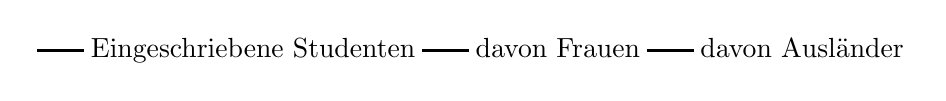
\begin{tikzpicture}
  \matrix[/pgfplots/every axis legend,at={(0,0)},anchor=north,draw=none] (L) {
    \sample{S1} & \node(T1){Eingeschriebene Studenten}; &
    \sample{S2} & \node(T2){davon Frauen}; &
    \sample{S3} & \node(T3){davon Ausl\"ander};\\};
  \reportpoint{L}{west}\reportpoint{L}{east}
  \reportpoint{S1}{center}\reportpoint{S2}{center}\reportpoint{S3}{center}
  \reportpoint{T1}{text}\reportpoint{T2}{text}\reportpoint{T3}{text}
\end{tikzpicture}
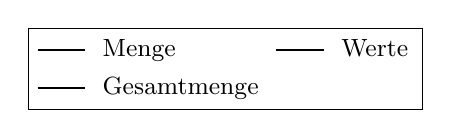
\begin{tikzpicture}
  \matrix[/pgfplots/every axis legend,at={(0,0)},anchor=north,font=\small,
      cells={anchor=west},column sep=4pt,row sep=2pt] (L) {
    \sample{S1} & \node(T1){Menge}; & \sample{S2} & \node(T2){Werte};\\
    \sample{S3} & \node(T3){Gesamtmenge};\\};
  \reportpoint{L}{west}\reportpoint{L}{east}
  \reportpoint{S1}{center}\reportpoint{S2}{center}\reportpoint{S3}{center}
  \reportpoint{T1}{text}\reportpoint{T2}{text}\reportpoint{T3}{text}
\end{tikzpicture}
\end{document}
